\documentclass{article}
\usepackage{graphicx} % Required for inserting images
\usepackage[backend=biber]{biblatex}
\addbibresource{references.bib}
\graphicspath{C:\Users\keyur\OneDrive\Desktop\IIT M\Acads\ID2090}
\title{ID2090 Assignment 4}
\author{Keyur Dhananjay Joshi \\ MM22B038 \\ Github ID: keyur18j }
\date{June 2023}

\begin{document}

\maketitle

\section*{Introduction}
The equation I have chosen is based on one of the most fundamental law of Physics. The person who has derived this equation is one of the greatest mathematicians of all times - \emph{'Sir Issac Newton'}. One of his most famous derivations is the \emph{Newton's Law of Universal Gravitation}. There were significant contributions by famous mathematicians- \emph{Galileo} and \emph{Kepler} in this Law. This law was majorly derived and proved around $17^\text{th}$ - $18^\text{th}$ century.

\section*{Newton's Law of Universal Gravitation}
According to Newton's Law of Universal Gravitation \cite{newton}, every particle in the universe attracts every other particle with a force that is directly proportional to the product of their masses and inversely proportional to the square of the distance between them.


\subsection*{Formula}
In scalar notation:
\begin{equation}
    \begin{math}
    F =  G \frac{m_1m_2}{R^2}
    \end{math}
\end{equation}
In vector notation:
\begin{equation}
    \vec{F} = -G\frac{m_1m_2}{r^2} \hat{r}
\end{equation}
In vector notation, we get a negative sign because the force is directed towards the object. 

Where, \newline
\(F\) is Gravitational Force \newline
\(G\) is Universal Gravitation Constant \newline
\(m_1\) and \(m_2\) are masses of two bodies \newline
\(R\) is the distance between the two bodies \newline

\begin{figure}
  \centering
  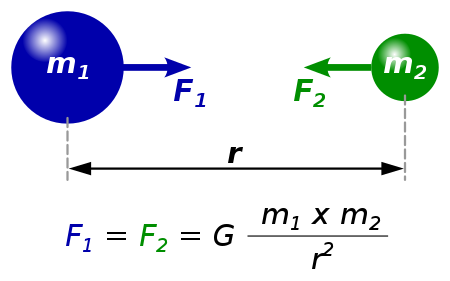
\includegraphics[width=0.5\textwidth]{Newtons law image.png}
  \caption{Gravitational Law}
  \label{fig:image}
\end{figure}


\section{Applications}
This Equation gives us the gravitational force between two bodies with known masses and distance between them. Here, value of \(G\) was determined experimentally and was found to be \(6.67430 * 10^{-11}\) \(m^{3} \cdot kg^{-1} \cdot s^{-2}\). 

\section{Plot}
This law follows the \emph{inverse square law}. It implies that it tends to zero rapidly as distance increase and tends. But the variation for \(r<R\) is different, where \(R\) is the Radius for the planet. This is a graph which shows variation of Gravitational Force as a function of distance from a planet.

\begin{center}
    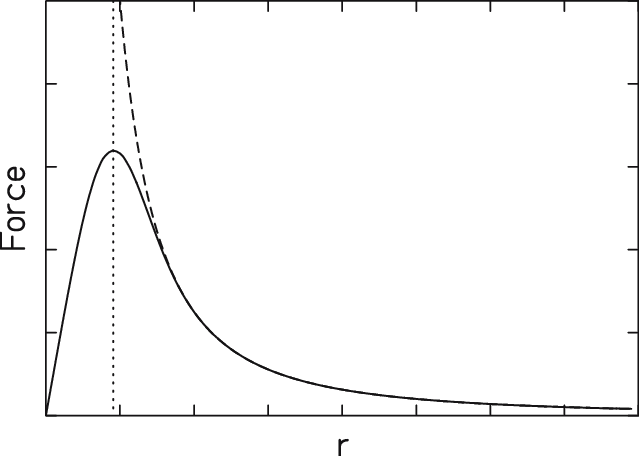
\includegraphics[width=0.6\textwidth]{newtons law graph.png}
\end{center}

\section{Why I chose this Equation?}
Many maths Giants Galileo, Kepler, Newton, Hooke have contributed to this equation. It nearly explained all the reasons for which supported the heliocentric solar system model. Even it is used now a days to compute trajectories of rockets, planets or even other comets and asteroids in the solar system. So, this is truly one of the most important equations in physics. 
\newpage
\printbibliography

\end{document}
